\documentclass[a4paper, 10pt, conference]{ieeeconf}
\usepackage[utf8]{inputenc}
\usepackage{graphicx}
\usepackage{amsmath}
\usepackage{amssymb}
\usepackage{url}
\usepackage{xcolor}
\usepackage{hyperref}
%
% ##########################
% include as many packages you need here
% ##########################
%
\usepackage{booktabs}
\usepackage{tikz}
\usetikzlibrary{positioning,arrows.meta}



%
% ##########################
% Do not change this header
% ##########################
%
\title{WACV 2027 UPAR Challenge\\ \textit{Fact sheet}}
\begin{document}
\maketitle
This is the fact sheet's template for the \href{https://vap.aau.dk/rws/challenge/}{WACV 2027 UPAR Challenge}. Please fill out the following sections carefully in a scientific writing style. Then, send the compressed project (in \texttt{.zip} format), i.e., the generated PDF, \texttt{.tex}, \texttt{.bib} and any additional files to \url{upar.challenge@gmail.com}.
%
% end of the header
%------------------
%





% ##########################
% Next, you are asked to fill in the required information
% (please, do not remove/change any item)
% ##########################
%
\section{Team details}\label{teamdetails}
\begin{itemize}
    \item Team leader name: Farrukh Ahmed Siddiqui
    \item Username(s) on Codabench: farrukh-siddiqui
    \item Team leader affiliation: Department of Artificial Intelligence, FAST-NUCES City Campus, Karachi, Pakistan
    % \item Team leader address:
    % \item Team leader phone number:
    \item Team leader email: farrukhsiddiqui.6465@gmail.com
    \item Name of other team members (and affiliation): Syed Muhammad Arham Tahir (Department of Artificial Intelligence, FAST-NUCES City Campus, Karachi, Pakistan), Syed Muhammad Hamza Naveed (Department of Artificial Intelligence, FAST-NUCES City Campus, Karachi, Pakistan)
    \item Team website URL (if any): none
    \item Competition track (mark with X one single option)\footnote{If you participated in more than one competition track, you need to share with the organizers one fact sheet per track.}:
    \begin{itemize}
        \item (X) Track 1: Pedestrian Attribute Recognition.
        \item ( ) Track 2: Attribute-based Person Retrieval.
        \item ( ) Track 3: Human Pose Estimation.
    \end{itemize}
\end{itemize}
We did not submit a paper to the RWS workshop.
%
% end of 'Team details'
%------------------
%





% ##########################
% Next, you are asked to fill in the required information
% Here, you are free to add figures and tables, and expand the default sections to better explain your method and contributions.
% ##########################
%
\section{Contribution details}
%

\subsection{Title of the contribution}
\textbf{Domain-generalised CLIP ViT-L/14 with leave-one-dataset-out model selection, WiSE-FT and a metric-aware set decoder.}

We fine-tune the image encoder of OpenAI CLIP ViT-L/14~\cite{radford2021clip} for the 40 UPAR attributes~\cite{Specker_2023_WACV}. Because the test domain is unseen, every design choice (backbone, WiSE-FT mixing weight, decoder) is made on leave-one-dataset-out (LODO) validation: three models are trained, each holding out one source dataset (Market1501, PA-100K, PETA) entirely. The contributions are (i) a text-initialised attribute head that starts fine-tuning from CLIP's zero-shot classifier, (ii) weight-space interpolation towards the zero-shot model (WiSE-FT~\cite{wortsman2022wiseft}) for robustness, and (iii) a per-image decoder that selects the attribute set maximising a first-order estimate of the challenge metric, tuned only on LODO predictions.

\subsection{Representative image / workflow diagram of the method}
Fig.~\ref{fig:pipeline} shows the pipeline.

\begin{figure}[h]
\centering
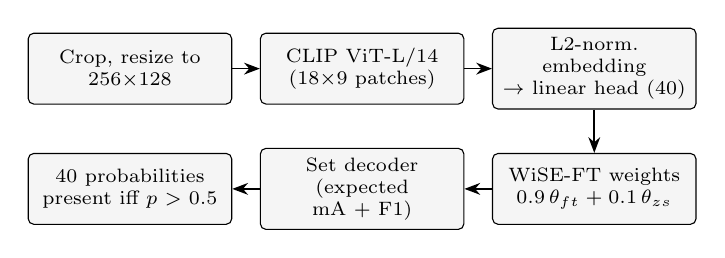
\begin{tikzpicture}[
  box/.style={draw, rounded corners=2pt, align=center, font=\scriptsize, minimum height=0.9cm, text width=2.35cm, fill=black!4},
  arr/.style={-{Stealth[length=2mm]}, semithick}]
\node[box] (a) {Crop, resize to\\256$\times$128};
\node[box, right=0.35cm of a] (b) {CLIP ViT-L/14\\(18$\times$9 patches)};
\node[box, right=0.35cm of b] (c) {L2-norm. embedding\\$\rightarrow$ linear head (40)};
\node[box, below=0.55cm of c] (d) {WiSE-FT weights\\$0.9\,\theta_{ft}+0.1\,\theta_{zs}$};
\node[box, left=0.35cm of d] (e) {Set decoder\\(expected mA + F1)};
\node[box, left=0.35cm of e] (f) {40 probabilities\\present iff $p>0.5$};
\draw[arr] (a) -- (b); \draw[arr] (b) -- (c); \draw[arr] (c) -- (d);
\draw[arr] (d) -- (e); \draw[arr] (e) -- (f);
\end{tikzpicture}
\caption{Inference pipeline. The head is initialised from CLIP text embeddings of a positive and a negative prompt per attribute; the WiSE-FT mixing weight and the decoder parameters are tuned on leave-one-dataset-out predictions.}
\label{fig:pipeline}
\end{figure}

\subsection{Detailed method description}
\textbf{Data and validation.} We use the provided train and validation splits of PA-100K, Market1501 and PETA (131{,}076 crops) and no other data. For model selection, three LODO folds are trained, each holding out one dataset entirely; the held-out (out-of-fold) predictions estimate performance on an unseen domain. The submitted model is trained once on all 131{,}076 crops with the same recipe. Across our four submissions the LODO estimate preserved the leaderboard ranking, at a roughly constant offset of about $+0.05$.

\textbf{Pre-processing.} Every crop is resized to 256$\times$128 (PIL bilinear) and normalised; inside the model it is resized (bilinear, antialiased) to 252$\times$126 so that it tiles into 18$\times$9 patches of 14 pixels. The 16$\times$16 position embedding of CLIP is bicubically resized to 18$\times$9.

\textbf{Architecture.} The CLIP ViT-L/14 image encoder (24 blocks, width 1024, QuickGELU, OpenAI weights) is re-implemented in plain PyTorch with the original parameter names; its features match \texttt{open\_clip} to within $2.3\cdot10^{-6}$ (verified on ViT-B/16, which shares the code). The class-token output passes through the final LayerNorm and the 768-d projection, is L2-normalised, and feeds a linear layer with 40 outputs. For each attribute $a$ we write a positive and a negative prompt (e.g.\ ``a surveillance photo of a pedestrian wearing a skirt or a dress'' / ``\dots wearing trousers or shorts''), encode them with the CLIP text encoder, and initialise the head weight as $w_a = 100\,(\hat t_a^{+} - \hat t_a^{-})$ with zero bias, i.e.\ the zero-shot classifier (mA $\approx 0.65$ before training). The text encoder is used only offline for this initialisation.

\textbf{Loss.} Binary cross-entropy with logits over the 40 attributes. The loss is masked for (source dataset, attribute) pairs with fewer than 5 positives in the training data (e.g.\ Market1501 has no brown, orange or pink upper body), because those zeros mean ``not annotated'' rather than ``absent''.

\textbf{Training.} 5 epochs, batch size 32, bf16 mixed precision, on one AMD RX~9070~XT (ROCm 7.1, PyTorch 2.13). The first epoch trains only the head (LP-FT~\cite{kumar2022lpft}), then the full network is fine-tuned. AdamW with weight decay 0.05 (not on norms, biases and embeddings); learning rate $2\cdot10^{-5}$ with layer-wise decay 0.8 per block, $10^{-3}$ for the head; linear warm-up over half an epoch followed by cosine decay; gradient clipping at norm 1.0; stochastic depth (drop path) 0.1, linearly increasing with depth; an exponential moving average of the weights (decay 0.999) is the evaluated and saved model. Images are sampled with replacement with probability proportional to $|D|^{-0.5}$ of their source dataset $D$, so PA-100K (68\% of the data) does not dominate. A full run (3 LODO folds + final model) takes about 4.5 hours.

\textbf{Augmentation} (on the GPU, no hue changes because 25 attributes are colours): horizontal flip ($p=0.5$); random scale $[0.85, 1.10]$, aspect $\pm15\%$ and translation up to $\pm6.5\%$ of the image size; low-resolution simulation ($p=0.4$; down-sampling to a height of 24--64\,px or by 0.25--0.6, then up-sampling); horizontal or vertical motion blur of 3--9\,px ($p=0.2$); JPEG re-encoding with quality 30--90 ($p=0.3$); contrast and saturation jitter of $\pm20\%$ and a brightness shift of $\pm0.2$ in normalised units; random erasing ($p=0.4$).

\textbf{WiSE-FT.} The submitted weights are $\theta = 0.9\,\theta_{\text{fine-tuned}} + 0.1\,\theta_{\text{zero-shot}}$, where $\theta_{\text{zero-shot}}$ is CLIP with the text-initialised head. The mixing weight was chosen on LODO from $\{1.0, 0.9, 0.8, 0.7\}$.

\textbf{Set decoder (post-processing).} With $q_a = \sigma(z_a/T)$ for logits $z_a$ and attribute priors $\pi_a$ (training positive rates, each dataset weighted equally), the mA gain of predicting $a$ positive is proportional to $g_a = q_a/\pi_a - (1-q_a)/(1-\pi_a)$. For each image and each set size $k = 1,\dots,20$ we take the top-$k$ attributes by
\begin{equation}
s_a(k) = \frac{w}{80}\,g_a + (1-w)\Big(\frac{\rho}{k} + \frac{1-\rho}{\sum_b q_b}\Big)\,q_a ,
\end{equation}
whose sum estimates the change in mA plus instance precision and recall, and keep the $k$ with the largest total. If no upper-body colour is chosen, the most likely one is added. Chosen attributes are output as $0.51 + 0.48\,q_a$ and the others as $0.49\,q_a$, so the platform's 0.5 threshold reproduces the decision. $T=0.85$, $w=0.5$, $\rho=0.45$ were selected by grid search on the LODO predictions; nested LODO (fit on two held-out datasets, score the third) gives 0.829 for the set decoder against 0.817 for per-attribute thresholds and 0.805 for a fixed 0.5 threshold.

\textbf{Inference.} \texttt{run.py} decodes images with 16 threads and runs batches of 128 in fp16 without test-time augmentation (flip TTA gained only $+0.001$ on LODO at twice the cost). The 29{,}248 test images took 101.5\,s on the A10.

\subsection{Challenge results}
Table~\ref{tab:results} reports our last submission (Codabench submission 1007093) as listed in the final leaderboard snapshot, where it ranks 31st of 89 entries. Table~\ref{tab:datasets} gives the per-dataset breakdown from the official scoring output.

\begin{table}[h]
\centering
\caption{Final leaderboard result (test set).}
\label{tab:results}
\setlength{\tabcolsep}{3.5pt}
\begin{tabular}{ccccccc}
\toprule
Avg & mA & Label F1 & Inst Acc & Inst Prec & Inst Rec & Inst F1 \\
\midrule
0.7856 & 0.7877 & 0.5504 & 0.6723 & 0.7531 & 0.8343 & 0.7835 \\
\bottomrule
\end{tabular}
\end{table}

\begin{table}[h]
\centering
\caption{Per-dataset results of the same submission.}
\label{tab:datasets}
\setlength{\tabcolsep}{3.5pt}
\begin{tabular}{lcccccc}
\toprule
Dataset & mA & Label F1 & Inst Acc & Inst Prec & Inst Rec & Inst F1 \\
\midrule
MEVID & 0.7335 & 0.4660 & 0.5965 & 0.7007 & 0.7768 & 0.7291 \\
Synth & 0.8419 & 0.6348 & 0.7480 & 0.8054 & 0.8917 & 0.8380 \\
\bottomrule
\end{tabular}
\end{table}

\subsection{Final remarks}
\textbf{Pros.} LODO validation predicted the ranking of all our submissions without any tuning on the test set. A vision-language backbone transfers markedly better than an ImageNet CNN (ConvNeXt-Tiny 0.7347, CLIP ViT-B/16 0.7605, CLIP ViT-L/14 0.7856 on the leaderboard). The decoder adds $+0.024$ on LODO at negligible cost, and the model runs in about a third of the time limit.

\textbf{Cons.} Attributes whose definition differs between the source datasets remain weak: Age-Young (test mA 0.50) is recognised with AUC 0.93--0.96 when Market1501 or PA-100K is held out but only 0.61 when PETA is held out, and the ``Other'' colours behave similarly. The decoder cannot repair a poor ranking. Most of the remaining gap is on MEVID (0.731 vs 0.840 on Synth). On LODO, a logistic stacker over label correlations, ensembling with ViT-B/16, zero-shot logit fusion and a weight soup of two ViT-L runs gave no improvement.


\section{Additional method details}
Please, reply if your challenge entry considered (or not) the following strategies and provide a brief explanation. For each question, mark with X one single option. \\

%
% mark with an X each question.
%
\begin{itemize}
%------------------------------------
\item \textbf{For the competition track associated with this fact sheet, you confirm that you have trained your model on the predefined datasets} (X) Yes, (~) No\\
%------------------------------------

%------------------------------------
\item \textbf{Did you use any pre-trained model:} (X)~Yes, (~)~No.\\ If yes, please detail (e.g., model architecture, training strategy, train data, etc.).\\
%
% include any additional comments here
%
OpenAI CLIP ViT-L/14~\cite{radford2021clip} (image--text contrastive pre-training on 400M web image--text pairs; not trained for pedestrian attribute recognition). The image encoder is fine-tuned as described above; the text encoder is used only once, offline, to initialise the attribute head.
%------------------------------------

%------------------------------------
\item \textbf{Did you use external data?} (~) Yes, (X) No\\
If yes, please detail:\\
%
% include your comments here
%
%------------------------------------

%------------------------------------
\item \textbf{Did you perform any data augmentation?} \\(X) Yes, (~) No\\
If yes, please detail:\\
%
% include your comments here
%
Horizontal flip, random scale/aspect/translation, low-resolution simulation (down- and up-sampling), motion blur, JPEG re-encoding, brightness/contrast/saturation jitter and random erasing; no hue changes (details in the method description).
%------------------------------------

%------------------------------------
\item \textbf{Did you use the provided validation set as part of your training set?} (X) Yes, (~) No\\
If yes, please detail:\\
%
% include your comments here
%
The submitted model is trained on the train and validation splits of all three datasets. Model selection used leave-one-dataset-out folds (train+val of two datasets for training, the third dataset held out).
%------------------------------------


%------------------------------------
\item \textbf{Did you use any regularization strategies/terms?} (X) Yes, (~) No\\
If yes, please detail:\\
%
% include your comments here
%
Weight decay 0.05, drop path 0.1, EMA of weights (0.999), layer-wise learning-rate decay, head-only first epoch (LP-FT), and WiSE-FT interpolation towards the zero-shot model.
%------------------------------------


%------------------------------------
\item \textbf{Did you use any pre-processing steps?} (X) Yes, (~) No\\
If yes, please detail:\\
%
% include your comments here
%
Resize to 256$\times$128 (internally 252$\times$126) and normalisation with CLIP statistics.
%------------------------------------


%------------------------------------
\item \textbf{Did you use any post-processing steps?} (X) Yes, (~) No\\
If yes, please detail:\\
%
% include your comments here
%
The per-image set decoder described above (temperature, priors and set selection maximising expected mA and instance F1), with one forced upper-body colour; no test-time augmentation and no use of test-set statistics.
%------------------------------------


%------------------------------------
\item \textbf{Did you use Vision Language Models (VLMs) of any kind?} (X) Yes, (~) No\\
If yes, please detail:\\
%
% include your comments here
%
CLIP ViT-L/14, a contrastive vision--language model: its image encoder is the fine-tuned backbone and its text encoder provides the head initialisation. No generative VLM is used.
%------------------------------------
\end{itemize}



\section{Code repository}
Link to a code repository with complete and detailed instructions so that the results obtained on Codabench can be reproduced locally. This includes a list of requirements, pre-trained models, and so on. Note, training code with instructions is also required. This is required for all participants to appear in the final ranking. \textbf{Organizers strongly encourage the use of docker to facilitate reproducibility}. \\

\textbf{Code repository:} \url{https://github.com/FarrukhSiddiqui/farrukh-upar2027-track1-submission}

\textbf{Trained weights:} \url{[WEIGHTS_URL]}




\bibliographystyle{IEEEtran}
\bibliography{references}
\end{document}
